\chapter{Methodology}

\section{Case Study: Telecommunication Company (AEM Fiber)}

We opted to model our framework in a real-world context by mapping the competences of a helpdesk employee at AEM Fiber \footnote{For privacy reasons we cannot declare the exact name of the company, so we will refer to it with the fictitious name "AEM Fiber" throughout this paper.}. AEM Fiber is an Italian telecommunications company with a keen interest in new technologies. This practical application aims to illustrate how our framework would operate within the context of a dynamic and forward-thinking organization.

The helpdesk employee's competences have been modeled based on the User Support role described in the e-Competence Framework (e-CF) \cite{ecompetenceframework}.
The e-CF is a reference framework for ICT competences that can be used in Europe by ICT companies to profile their professionals, managers, and human resources employees.\label{sec:ecompetence-framework}
Each role described in the European e-Competence Framework is organized into four sections:
\begin{itemize}
      \item Section 1 describes the company areas: PLAN - BUILD - RUN - ENABLE - MANAGE. PLAN and ENABLE represent the strategic areas. BUILD concerns the development and realization of products or services and RUN focuses on the provision, support, and maintenance of released solutions. Both provide the operational subprocesses through which companies take action and get things done. MANAGE represents the daily operations of companies to administer and improve their business.
      \item Section 2 defines a set of reference e-Competences for each role, with a general description for each competence.
      \item In section 3 there are examples of skills related to the section 2 competences.
      \item In section 4 there are examples of knowledge related to the section 2 competences.
\end{itemize}
In this framework, competence is defined as a demonstrated ability to apply knowledge and skills to achieve observable results.
In e-CF, the \textit{level} concept refers to levels of proficiency in a certain competence. A proficiency level integrates three aspects: context complexity, autonomy, and behavior. Autonomy ranges from 'Follow instructions' to 'Make personal choices'. Context complexity extends from 'Structured - Predictable' situations to 'Unstructured - Unpredictable' situations. Behavior in this context represents an observable outcome of attitude and ranges from 'ability to apply' to 'ability to conceive'.
For this paper we decided to evaluate the User Support role, so we used the corresponding role description in the framework to extrapolate the competences we needed.
Then, we had to tailor the framework to our specific case study. To this end we will now describe the AEM Fiber structure, focusing on the User Support role, to better explain our mapping choices.

The company has two main departments: the technical department and the administrative department. We will not consider the administrative department since the User Support role belongs to the first one. The technical department branches into three levels:
\begin{itemize}
      \item In the first level, the employee has to answer incoming calls from AEM Fiber clients who report an issue with the services provided by the company. If the reported issue can be easily solved, the employee is expected to assist the client in resolving the problem. If the issue is too complex, the employee has to escalate the client's call to the second level. In addition, if it is needed, the employee has to call back the client to solve the problem.
      \item The second level employees have to deal with more complicated client issues, escalated from the first level.
      \item The third level is the one that is involved in dealing with configurations or operations that affect a macro area of customers. We will not discuss it in detail.
\end{itemize}

\begin{center}
      \begin{figure}[ht]
            \centering
            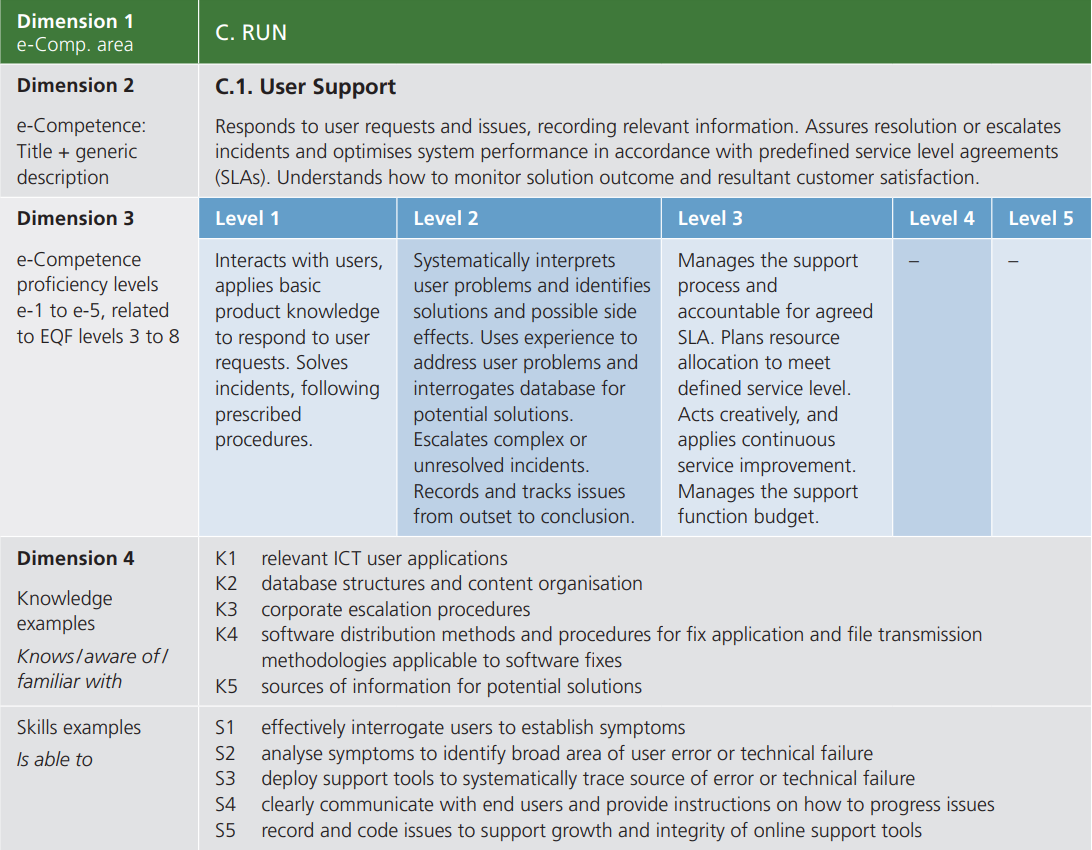
\includegraphics[width=0.9\textwidth]{user_support_ecf.png}
            \caption[short]{e-CF User Support role description}
            \label{fig:usersupportecf}
      \end{figure}
\end{center}


Figure \ref{fig:usersupportecf} illustrates the e-CF description of a technical role, presenting information in a clear and standardized manner. The left side of the figure is divided into several sections, as previously discussed. The first two sections provide a brief description of the role, emphasizing its connection to a specific business phase; in this specific figure, it is the operational phase known as RUN, indicative of day-to-day operations. Following that, the proficiency levels associated with the role are detailed. These levels can be roughly compared to the AEM Fiber levels, offering a standardized way to understand skill proficiency. The last element of the figure is a list of examples highlighting the essential knowledge and skills expected from an individual in the user support operator role.\\

Based on the indications of the domain expert, we determined that each AEM Fiber employee has to know how to deal with these issues, as presented in Figure \ref{fig:aemfibertasks}, according to their proficiency level: Configuration hosting mail, Connectivity disservice, POTS disservice, Input/output hosting mail, Connectivity degradation, SPAM, POTS degradation, VOIP disservice, VOIP degradation. The tasks in Figure \ref{fig:aemfibertasks} are in descending order of difficulty and the ability to solve them differs according to their difficulty level.

\begin{center}
      \begin{figure}[ht]
            \centering
            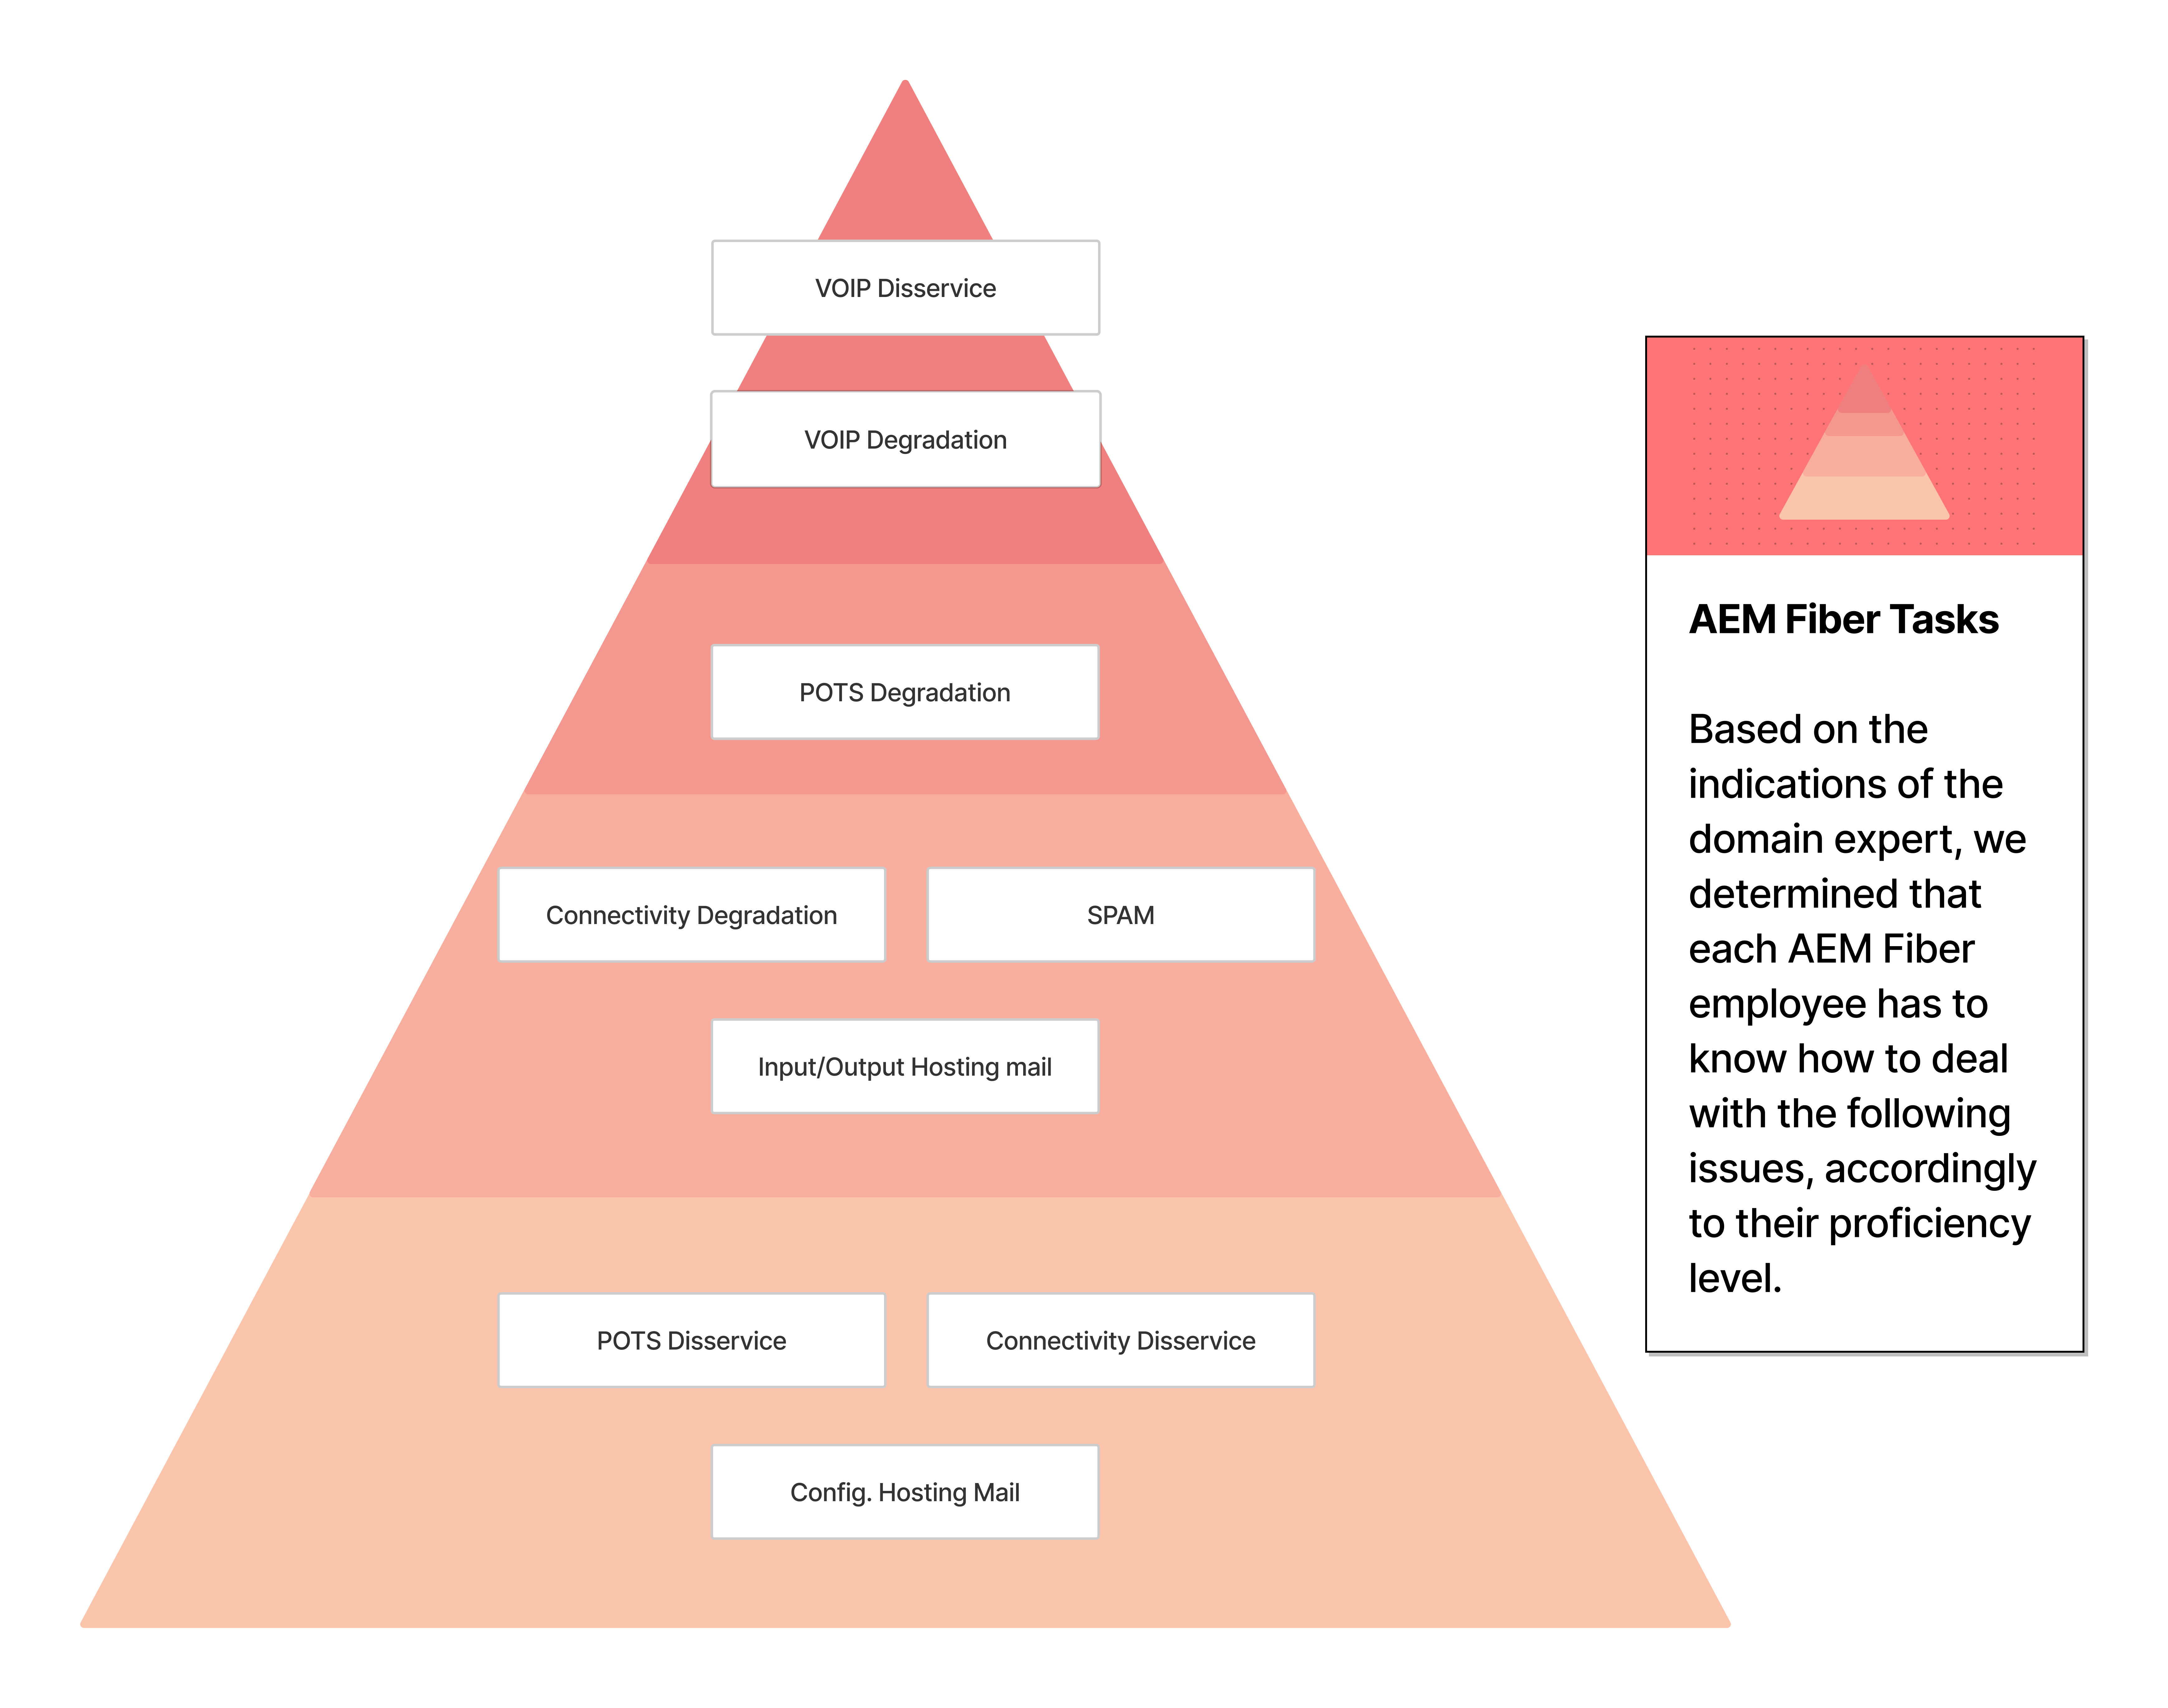
\includegraphics[width=0.9\textwidth]{aemfiber_tasks.png}
            \caption[short]{AEM Fiber task complexity pyramid}
            \label{fig:aemfibertasks}
      \end{figure}
\end{center}
\newpage

\section{Current AEM Fiber customer support workflow}

In Figure \ref{fig:aemfiberworkfloworiginal} we present the current AEM Fiber user support workflow process. In chapter \ref{sec:discussion} we will modify this workflow by adding the competence mapping phase, based on the results obtained during the experimental evaluation.

\subsection*{Call creation phase}

\begin{enumerate}
      \item Customer C calls the company support service to require assistance through the available communication channels.
      \item C is informed that the call will be recorded.
      \item The inbound call is assigned to Employee E.
      \item The dialogue between C and E is recorded.
      \item The call ends.
\end{enumerate}

\subsection*{Call update phase}

\begin{enumerate}
      \item Either Customer C or Employee E calls to provide/require updates on the reported issue.
      \item C is informed that the call will be recorded.
      \item The dialogue between C and E is recorded.
      \item The call ends.
\end{enumerate}

\begin{center}
      \begin{figure}[ht]
            \centering
            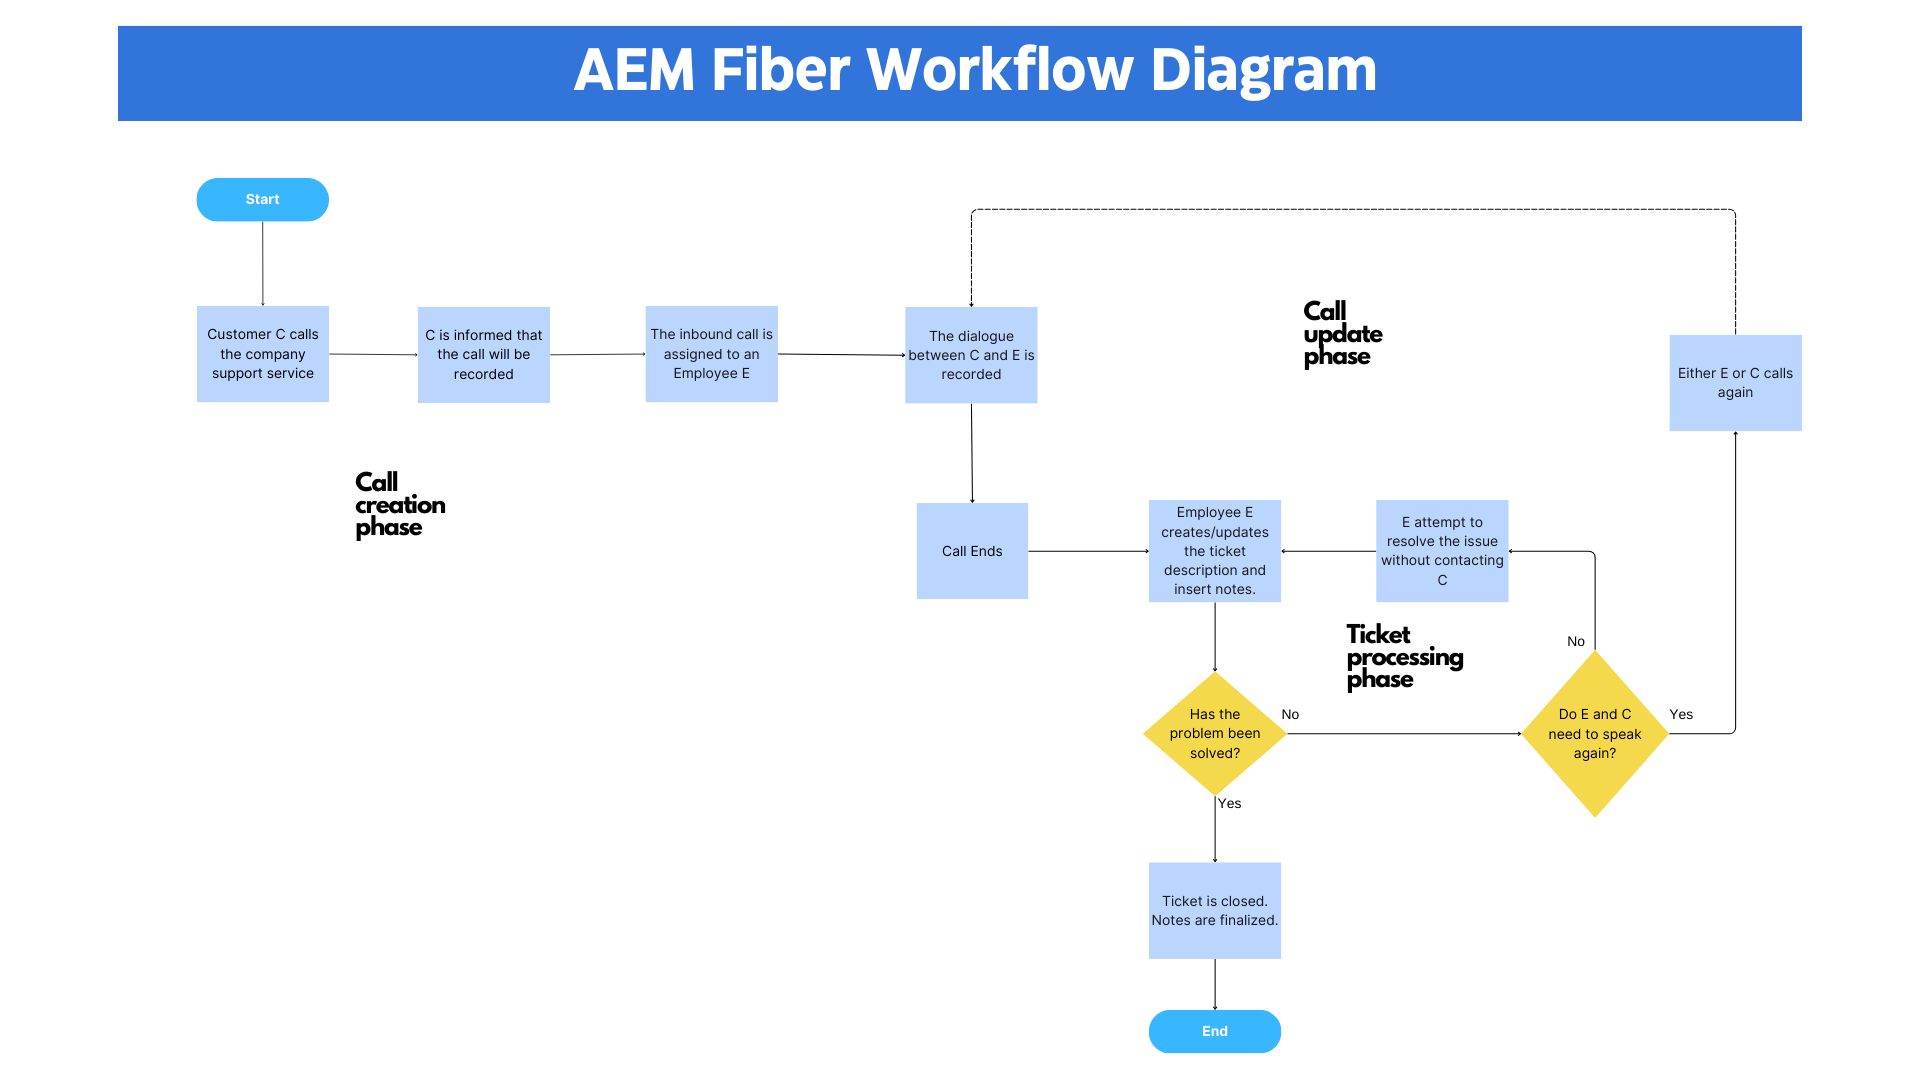
\includegraphics[width=1\textwidth]{workflow_original.png}
            \caption[short]{AEM Fiber customer support workflow}
            \label{fig:aemfiberworkfloworiginal}
      \end{figure}
\end{center}

\subsection*{Ticket processing phase}

\begin{enumerate}
      \item At the end of the first call (Call creation phase), employee E creates the ticket description.
      \item If needed the ticket is escalated from level 1 to level 2.
      \item After each operator's attempt to solve the issue or after any update call to/from the customer (Call update phase), new working notes are added to the existing ticket.
      \item When the problem has been solved and the customer is satisfied, notes are finalized and the ticket is closed.
\end{enumerate}

\section{Competence mapping in AEM Fiber}

Currently, AEM Fiber promotion system lacks a formal structure. Employees move up the levels based on management's assessment of their proficiency in resolving client issues and their ability to articulate themselves effectively. Typically, this advancement occurs after gaining experience within the company and by working on similar tasks daily. The decision on promotions heavily relies on the subjective judgment of the department manager, coupled with statistical data: the duration of customer calls, the number of resolved tickets, and the ticket categories are some of the metrics considered. However, these metrics only provide a partial view of employee competences and do not capture many aspects of their work. As a result, the manager's perspective plays a crucial role in the decision-making process. Additionally, the time an employee has spent at the company has a significant impact on promotion considerations.\\

As described in section \ref{sec:proposedframework}, our framework would extend the knowledge of the company on employee abilities, effectively improving the promotion system by incorporating a more comprehensive set of factors. Specifically, to evaluate the efficiency of a Large Language Model in the context of competence mapping we have decided to focus on a set of User Support macro-competences. Initially, we assess communication skills. This involves a detailed analysis of call transcripts handled by operators, utilizing the model to understand conversational dynamics. The objective is to evaluate the operators' proficiency in maintaining a friendly and clear communication style during calls. Subsequently, we delve into the evaluation of technical competences. This entails analyzing the user's request description to categorize it into specific subcategories based on ticket content. For instance, a "Hosting" ticket might be classified into subcategories like "Configuration Hosting Email" or "SPAM." By quantifying the successful resolution of tickets in each subcategory, we can comprehend the individual operators' skills. Each subcategory is also associated with a predefined difficulty level, as previously mentioned. Lastly, our framework includes an evaluation of problem-management competences. This involves analyzing the working notes generated by operators during the ticket resolution process to assess their ability to efficiently solve problems. While these three competences form the initial focus of our evaluation, it is important to acknowledge that additional competences may be identified. Given the academic nature of this paper, we are empirically testing and validating these competences within our proposed framework.

\section{Experimental evaluation}

We decided to use a transformer model for our tasks since it is the state-of-the-art architecture for NLP.
Due to the task at hand, we needed a generative model and decided to use GPT (Generative Pre-trained Transformer) thanks to its effectiveness at Closed Book Question Answering and Common Sense Reasoning.
In particular, we have chosen GPT3.5 because it was easily accessible, pre-trained on a vast set of examples, and ready to use. Since we couldn't access AEM Fiber data, we had to use external datasets for our experiments. We used \href{https://zenodo.org/records/4274454}{I-BiDaaS TID Synthetic Call Centre Dataset} to evaluate the communication competence and \href{https://data.milwaukee.gov/dataset/callcenterdatahistorical/resource/abdfe983-e856-40cd-bee2-85e78454344a}{Milwaukee City Call Center Dataset} for the technical competence evaluation. Together with the domain expert, we generated the working notes used to evaluate the problem management competence.

\subsection{Dataset description}
The first dataset is a simulated dataset comprising several simulated customer interactions with an agent representative, with both roles performed by actors. The scripting, both from customer and agent, aims to develop typical scenarios by Telco-oriented call center operations. Each record contains a transcription obtained by an automatic speech recognition system; the use of an automatic speech recognition system leads to dealing with some errors in the text (eg. incorrect transcription, missed speech parts)

\begin{quote}
      \label{transcription-nine}
      Tech: Movistar, good afternoon. This is Toledo speaking. Please tell me how I can assist you.

      Customer: Hello, good afternoon. I wanted to inquire about my current plan. I have one gigabyte of internet, and I want to know when I'll have the regular speed again after the usage is reset.

      Tech: Sure, in terms of billing cycles, your plan's usage resets from the 18th to the 17th of each month. I can check for you. The next reset will occur on the 18th of December, and you actually have two gigabytes included in your plan.

      Customer: I see. And if there hasn't been any usage yet?

      Tech: Let me check. Could you please provide me with the phone number for the other query?

      Customer: It's three four one nine eight zero five zero four nine eight.

      Tech: Alright. Let me check that line. Yes, that line ending in eighteen hasn't used any data yet.

      Customer: Yes, that's right. It's for my father, he has a non-internet phone. Is there any way to connect my line to his?

      Tech: I see. Well, if both lines have the same account holder, we can activate a shared data service at no additional cost. This way, you can share the data between the two lines.

      Customer: That's perfect. That's perfect.

      Tech: Alright, then. I'll activate it for you in just a moment, if you don't mind waiting.

      Customer: Okay.

      Tech: It's done for you now. In about five minutes, you'll be able to call and activate the service. So, both lines will have a total of four gigabytes to share.

      Customer: That's great. Thank you very much.

      Tech: You're welcome. Do you have any other questions or anything else we can help you with?

      Customer: No, just that.

      Tech: Alright, then. Thank you very much for the call. It was a pleasure assisting you.

      Customer: Very kind of you.

      Tech: Just a moment. They will call you to gather feedback on the service. Whenever you're available, feel free to provide your feedback. Have a good day.

      Customer: Thank you, you too.

      Tech: Thank you.
\end{quote}

In this scenario, the operator demonstrated kindness and effective communication skills in explaining information to the customer. Throughout the entire conversation, the operator maintained a professional and friendly approach. They were articulate in their explanations and successfully persuaded the customer to activate an additional service. From the perspective of customer satisfaction, it's evident that the customer was content by the conclusion of the conversation. This follows the guidelines of the company as explained by the domain expert. To better evaluate the model's ability to identify negative behaviors, we added some records to the dataset. These records featured actors simulating uncooperative customer-operator interactions, which required the model to recognize and respond to negative behaviors. An example of negative behavior is the following:

\begin{quote}
      Customer: Okay, okay. But is it for the same thing, or are they removing some service?

      Tech: No, we're not removing or adding any services. God how many time do I have to say this. It's for the same thing you have.

      Customer: Okay, okay no need to get agitated.

      Tech: Deal with it. Do you have any other questions?

      Customer: No, no.
\end{quote}

In this case, the operator is unclear and becomes unfriendly when the customer asks to clarify, which in turn makes the customer visibly uncomfortable. Such behavior clearly violates AEM Fiber guidelines and must be avoided or reported.

The second dataset contains information from the Milwaukee Call Center. It has six columns:
\begin{itemize}
      \item CREATION\_DATE: This shows when each request or call was made.
      \item OBJECT\_DESC: This column includes the location of the call, with the street address in Milwaukee, Wisconsin.
      \item TITLE: It categorizes each call into different categories, such as "Garbage Cart: Damaged."
      \item CLOSED\_DATETIME: This column records when the reported issue was resolved or closed, if applicable.
      \item CASE\_CLOSURE\_REASON\_DESCRIPTION: It explains why each case was closed, providing context for the resolution.
\end{itemize}
The dataset covers various issues, including garbage collection problems, street maintenance, and sanitation concerns. It is a record of interactions and issues reported to the Milwaukee Call Center, mirroring the issue report in our analyzed company.
\begin{center}
      \renewcommand{\arraystretch}{1.5}
      \begin{tabularx}{\textwidth}{l|X}
            \toprule
            TITLE           & CASE\_CLOSURE\_REASON\_DESCRIPTION                                                                                                                                                                                                                                                                                                                               \\
            \midrule
            All Other Signs & On Kearney St, there is a “No Left Turn” sign that was put up during the state fair, which I believe was intended to be temporary. The attached image shows where the sign is, although the “No left turn” sign is not present in the picture.                                                                                                                   \\
            \hline
            Pothole         & Heading southbound, in the right turn lane.                                                                                                                                                                                                                                                                                                                      \\
            \hline
            Pothole         & There was a chunk of pavement that popped out, looked like the resulting hole was beside a manhole in the southbound lane (76th). I believe the location of the pothole is within 20 ft of Stevenson St intersection. The chunk of pavement was no longer in traffic later in the day when I drove past again later in the day, so that aspect is not a concern. \\
            \hline
            Area Dark       & No light for a few months ago.                                                                                                                                                                                                                                                                                                                                   \\
            \hline
            One Way Sign    & Northbound on 76th, at O'Connor. One Way sign top bolt missing and sign is falling down. Attached picture shows the sign needing attention, although it is not falling down in the picture as it is an older picture from Google maps.                                                                                                                           \\
            \bottomrule
      \end{tabularx}
\end{center}

In AEM Fiber, the operators initiate their task by creating a summary equivalent to the OBJECT\_DESC value. After interacting with the customer, each operator is required to articulate the problem in a ticket description and select the relevant category. Accurate classification of each ticket holds significant importance for AEM Fiber, as it provides a clear insight into the company issues. Furthermore, a more detailed classification, including subcategories within each main category, would enhance the ability to evaluate each employee's performance based on their successfully resolved tickets.
For the third competence we tried searching for datasets that could contain transcriptions of work notes, but we couldn't find any that met our requirements. That's why we decided to generate our own work notes, thanks to the suggestions given by the domain expert about their structure and their general content. In particular, we wrote these notes directly in Italian language since AEM Fiber is an Italian company: in the real case, in fact, the operators write the notes in Italian.
Each work note contains the date, name of the technician who wrote the note, and the relative content; in particular, the latter contains all the steps of the problem management process. The domain expert told us that usually, the operators don't follow a proper structure while writing these notes. \label{sec:datasetProblemManagement}
Here we present some work note examples (translated into English).
\begin{itemize}

      \item First example

            14/09/23 08:00\\
            Operator 1\\
            Taken in charge, starting to check\\

            14/09/23 08:30\\
            Operator 1\\
            The line is working correctly, but the router is malfunctioning. Proceeding with replacement of it.\\

            15/09/23 11:30\\
            Operator 1\\
            Customer has received the router and confirms proper functionality.
\end{itemize}
In this case, the operator \textit{correctly} understands that the client's problem is about the router; that's why he decides to replace it. This perfectly fits with the company's guidelines and, since he also understood immediately the problem, this is an example of good problem management.
\begin{itemize}
      \item Second example

            14/08/2023 15:00\\
            Operator 4\\
            I take charge of the ticket.\\

            14/08/2023 15:15\\
            Operator 4\\
            The customer reports having slow connection only with wifi devices, but upon checking with tools, it seems there is an issue at the central office level. I involve the external technician so they can inspect the external central office.\\

            15/08/2023 16:00\\
            Operator 4\\
            Following the inspection of the external central office, the external technician informs me that there is no problem detected up to the main telephone socket, indicating that the issue is related to the internal installation. I contact the customer and agree on the replacement of the router.\\

            17/08/2023 10:30\\
            Operator 4\\
            The customer has received the router and connected it. They attempt a browsing test and report that it is working correctly. I ask them to monitor it and contact us in case of any issues. The closure of the report is agreed upon.
\end{itemize}

In this case, the operator \textit{wrongly} interprets the problem as an external one; this leads to the technician being sent to the central office unnecessarily. This is a serious issue for AEM Fiber because it means losing time and paying the external technician without him solving a real problem. So this is a bad example of problem management.